\chapter{Aplicația mobilă și infrastructura aplicației}
\label{cap:cap3}

\section{Aplicația Android}
Aplicația Android servește drept mediu de interacțiune cu modelul discutat în capitolul anterior. Aceasta este scrisă cu ajutorul limbajului \textbf{Kotlin} \cite{kotlin}, utilizând biblioteca de instrumente pentru dezvoltare, \textbf{Jetpack Compose} \cite{jetpackcompose}. Detecțiile au loc la nivel local, modelul fiind încărcat pe dispozitivul Android cu ajutorul \textbf{PyTorch Mobile}. Interfața pentru cameră este oferită de biblioteca \textbf{CameraX} \cite{camerax}, iar cererile \textit{HTTP}, transmise prin protocolul securizat \textit{HTTPS}, sunt facilitate de biblioteca \textbf{Retrofit} \cite{retrofit}. Ecranele prezentate în acest capitol funcționează pe baza unei stive gestionate cu ajutorul unui obiect de tip \textit{NavController}. În continuare, detaliem structura și fluxul logic al aplicației.

\textbf{Ecranul de bun-venit}. După deschiderea aplicației, utilizatorul este întâmpinat de ecranul de bun-venit (Figura~\ref{fig:welcome_screen}), unde îi sunt prezentate trei opțiuni: \textit{Sign In} (autentificare), \textit{Sign Up} (crearea unui cont nou) sau \textit{Skip and use offline} (simpla detectare a literelor). Aplicația afișează acest meniu doar în cazurile în care utilizatorul nu este autentificat sau este autentificat, dar dispozitivul nu este conectat la internet.


\textbf{Utilizarea fără conexiune la internet}. Această opțiune oferă  posibilitatea de a detecta literele fără autentificare, pentru a asigura o experiență cât mai plăcută și accesibilă utilizatorilor care își doresc să acceseze doar funcția de traducere. Aplicația încarcă modelul în memorie și încearcă să detecteze mâini afișate pe ecran cu ajutorul algoritmului MediaPipe Hands. Odată ce o mână este detectată, este decupat un dreptunghi care încadrează mâna și transmis mai departe către modelul responsabil pentru detecția literei. În cazul în care este detectat un semn valid, este afișată litera recunoscută (Figura~\ref{fig:offline_valid_detection}), iar în caz contrar, este afișat caracterul „-” (Figura~\ref{fig:offline_invalid_detection}).


\begin{figure}[H]
  \centering
  \begin{subfigure}{0.2\textwidth}
    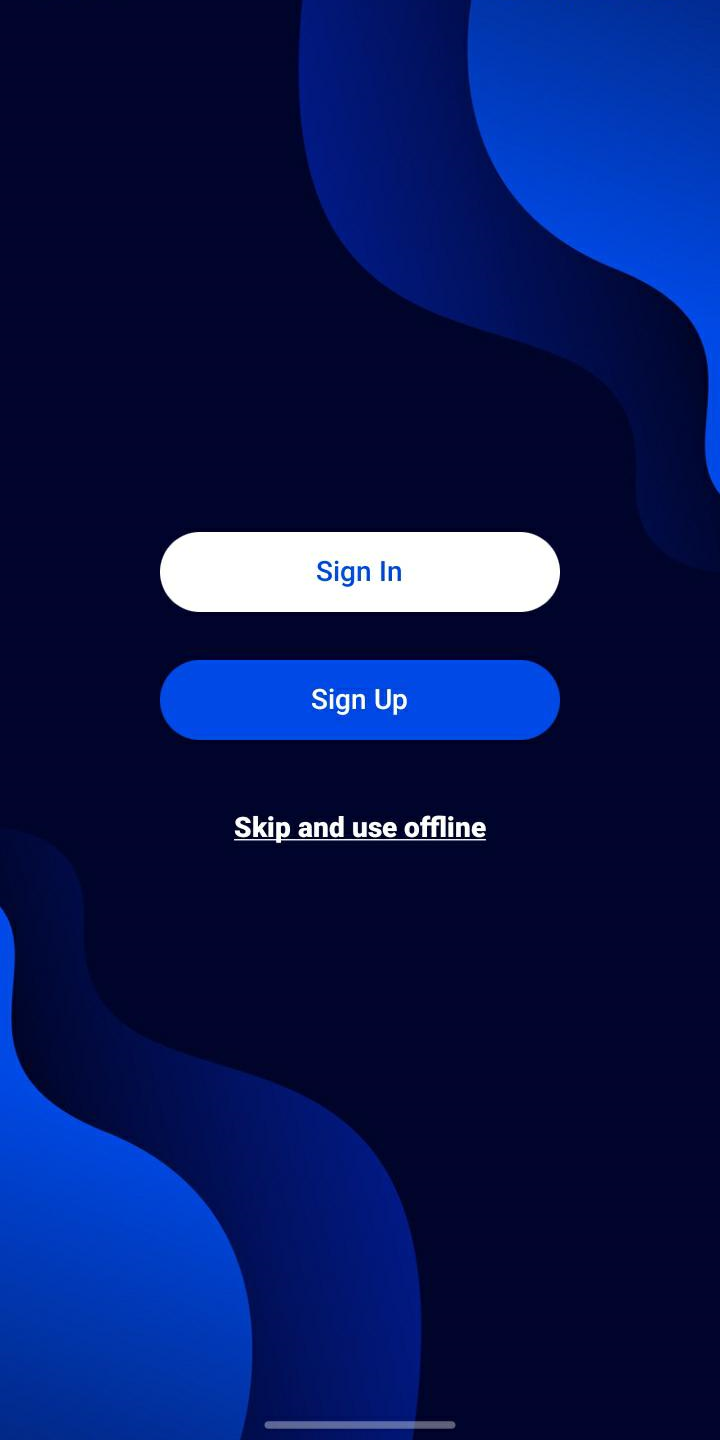
\includegraphics[width=\linewidth]{images/3-aplicatia-android/welcome_screen_android_app.png}
    \caption{}
    \label{fig:welcome_screen}
  \end{subfigure}
  \begin{subfigure}{0.2\textwidth}
    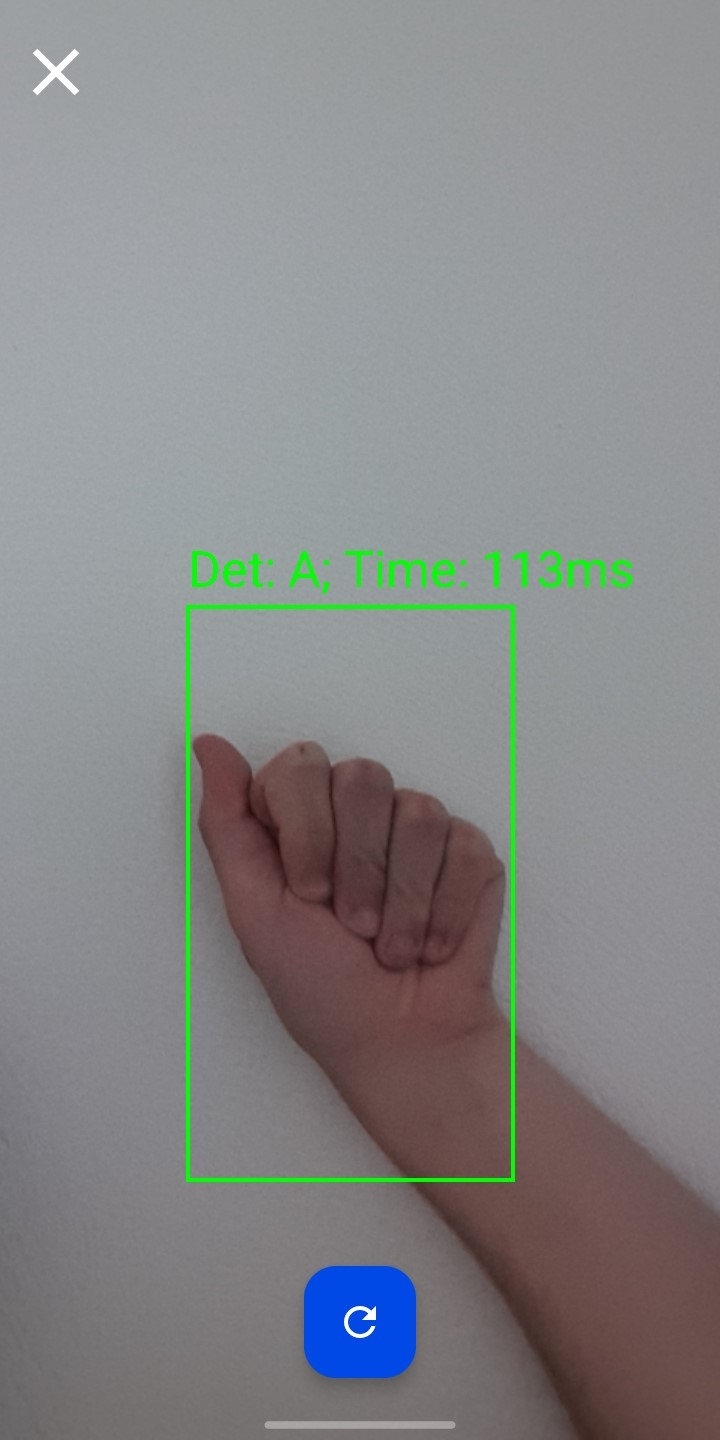
\includegraphics[width=\linewidth]{images/3-aplicatia-android/ffa_detection.jpeg}
    \caption{}
    \label{fig:offline_valid_detection}
  \end{subfigure}
  \begin{subfigure}{0.2\textwidth}
    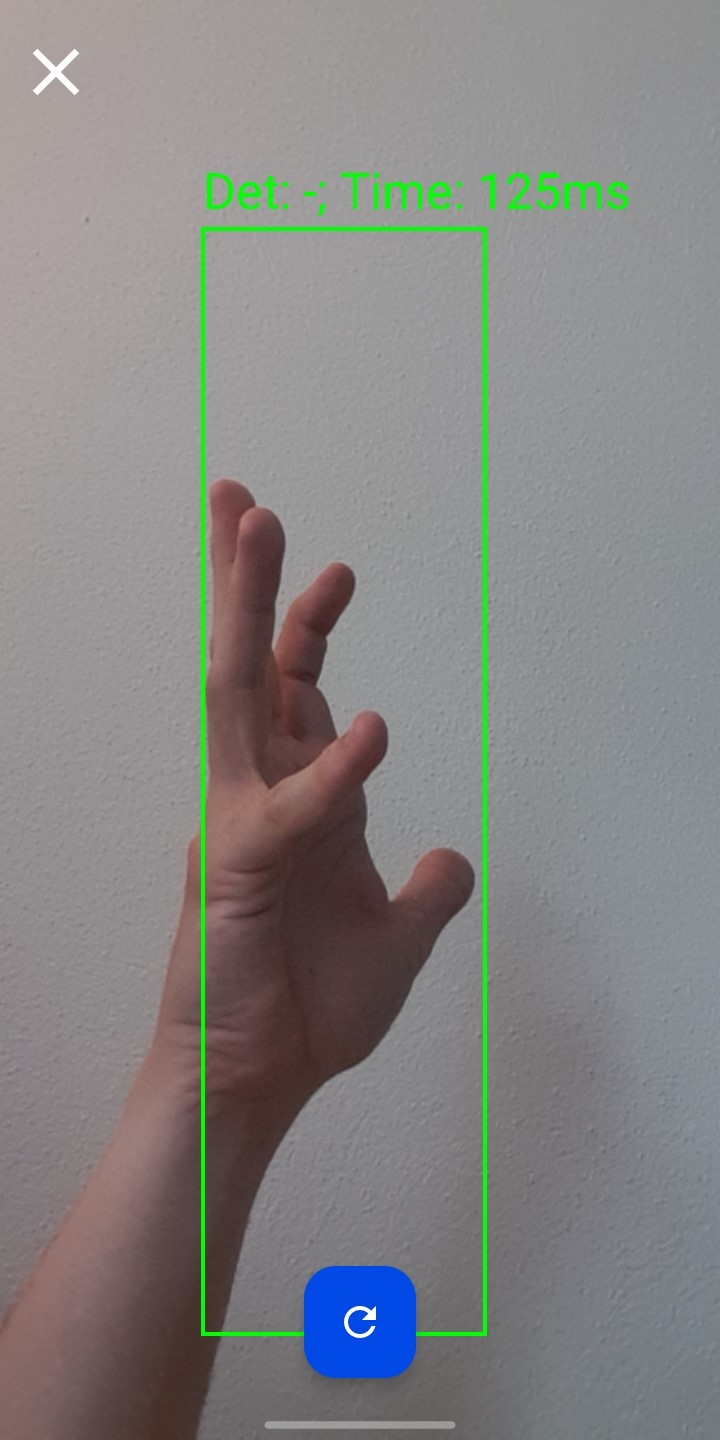
\includegraphics[width=\linewidth]{images/3-aplicatia-android/ffa_invalid_detection.jpeg}
    \caption{}
    \label{fig:offline_invalid_detection}
  \end{subfigure}
  \caption[Ecranele inițiale ale aplicației]{\textbf{Ecranele inițiale ale aplicației}. \textit{Ilustrăm ecranele inițiale ale aplicației. (a) ilustrează ecranul de bun-venit, unde sunt prezente butoanele de Sign In, Sign Up și Skip and use offline; (b) ilustrează modul de detecție în lipsa conexiunii la internet; palma detectată de MediaPipe Hands este încadrată în chenarul verde, deasupra căruia utilizatorul este înștiințat ca a fost detectată litera A, într-un timp de 113ms; (c) ilustrează momentul în care utilizatorul afișează un semn invalid.}}
  \label{fig:welcome_screen_offline_det_screen}
\end{figure}

\textbf{Autentificarea utilizatorilor}. Utilizatorul are posibilitatea de a crea un cont nou, de a se conecta cu datele sale, de a schimba parola și de a se deconecta.

Pentru început, utilizatorul apasă butonul de Sign Up, pentru a introduce adresa de email și parola noului cont (Figura~\ref{fig:sign_up_screen}). După o validare a câmpurilor, aplicația trimite datele către server. În cazul în care serverul oferă un răspuns pozitiv, utilizatorului îi este afișat ecranul de validare a adresei de email (Figura~\ref{fig:validation_screen}). În acest pas, utilizatorul află că are timp 5 minute pentru a introduce un cod primit pe email cu scopul de a confirma adresa. În urma unui răspuns valid din partea serverului privind codul de validare introdus, utilizatorul este înștiințat și redirecționat către ecranul de start, de unde se poate conecta cu noul său cont.


În urma apăsării butonului de Sign In, este afișat un ecran care oferă posibilitatea de a introduce datele contului (Figura~\ref{fig:sign_in_screen}), care sunt transmise către server pentru validare. În cazul unui răspuns pozitiv, utilizatorul este direcționat către meniul principal, unde poate opta pentru începerea unei sesiuni de antrenament în învățarea alfabetului ASL. Mai mult decât atât, odată cu răspunsul pozitiv, dispozitivul primește un \textbf{JSON Web Token} (JWT) \cite{jwt}, denumit token de acces, alături de un token de reîmprospătare. Detalii despre această metodă sunt oferite în Secțiunea~\ref{sec:server_app}.


În cazul în care utilizatorul își uită parola, acesta poate face o cerere de schimbare a parolei, care constă în introducerea adresei de email către care sunt trimise instrucțiunile pentru resetare (Figura~\ref{fig:forgot_password}).

\begin{figure}[H]
  \centering
  \begin{subfigure}{0.2\textwidth}
    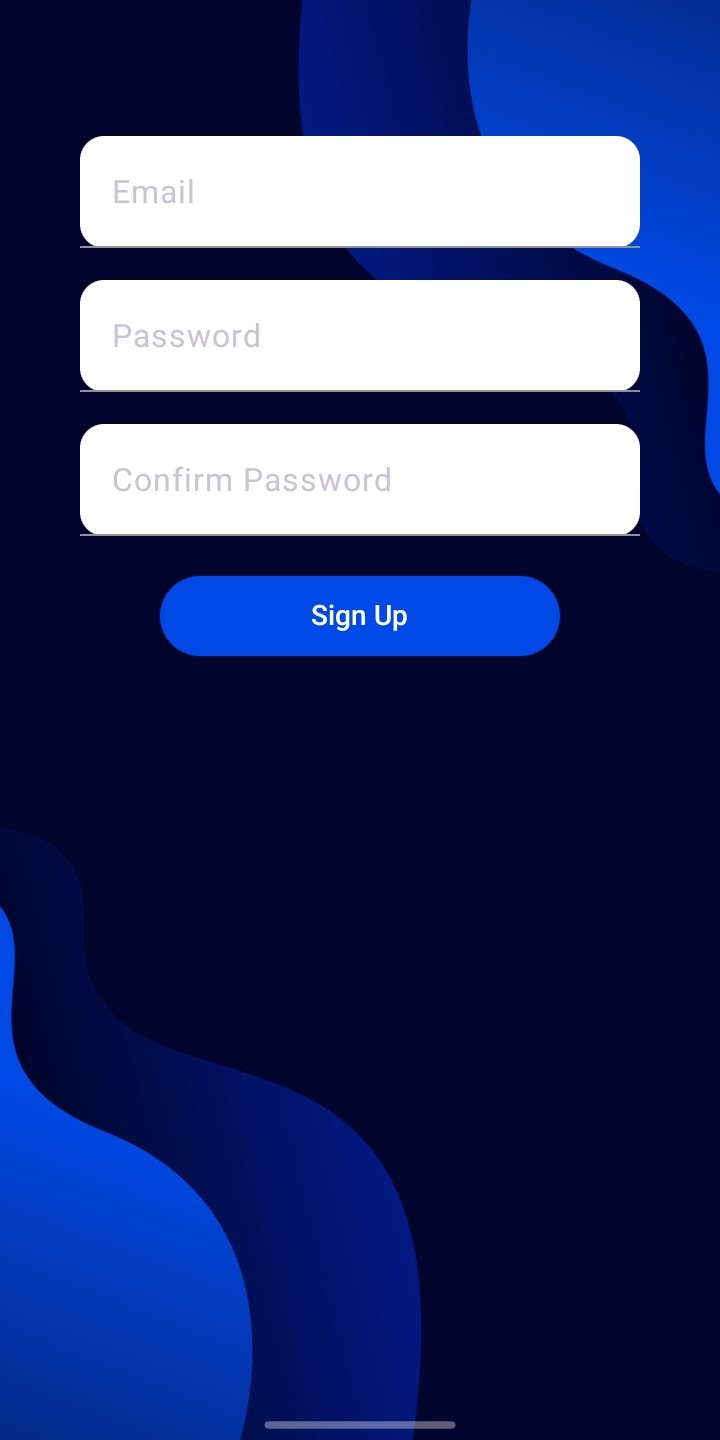
\includegraphics[width=\linewidth]{images/3-aplicatia-android/sign_up_screen.jpeg}
    \caption{}
    \label{fig:sign_up_screen}
  \end{subfigure}
  \begin{subfigure}{0.2\textwidth}
    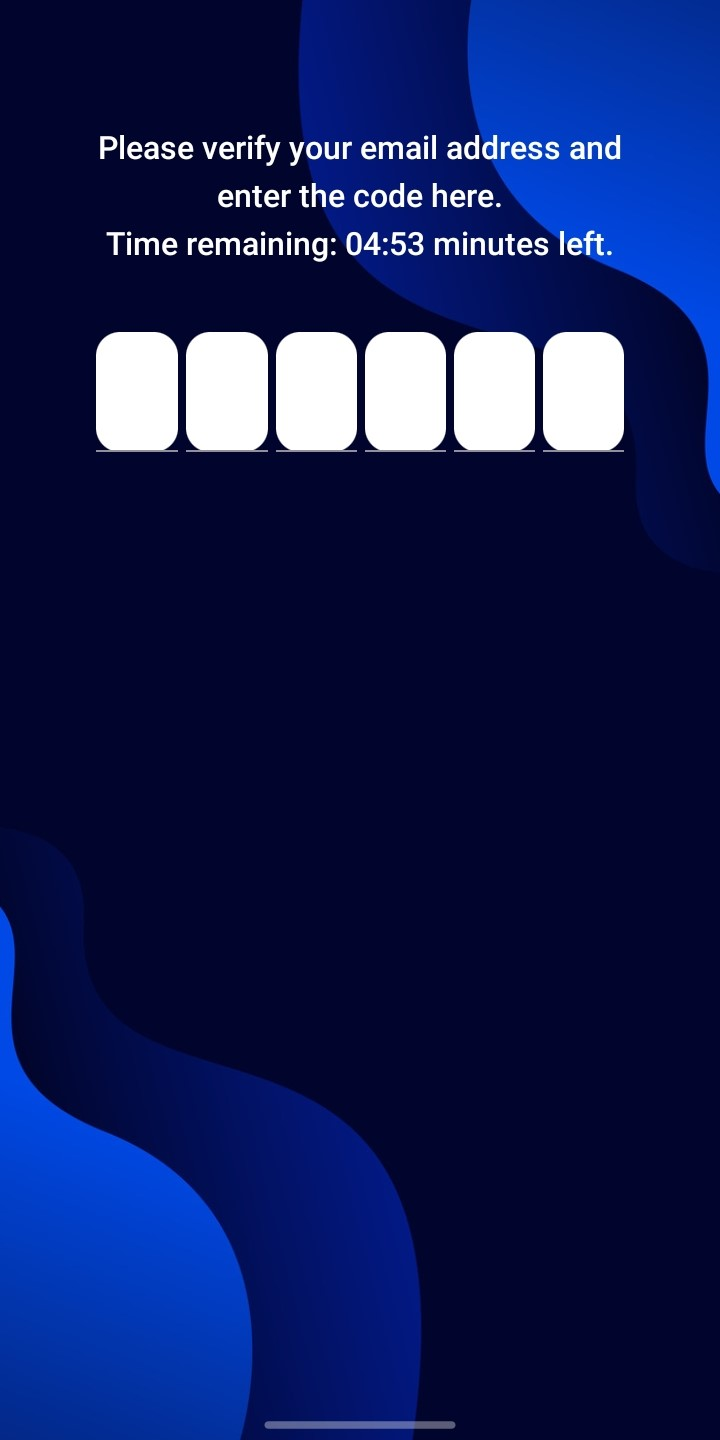
\includegraphics[width=\linewidth]{images/3-aplicatia-android/validation_code_screen.jpeg}
    \caption{}
    \label{fig:validation_screen}
  \end{subfigure}
  \caption[Crearea unui cont nou]{\textbf{Crearea unui cont nou}. \textit{Ilustrăm procesul de creare a unui cont nou. (a) ilustrează cele trei câmpuri necesare creării unui nou cont: email, parola, confirmarea parolei; (b) ilustrează înștiințarea utilizatorului de timpul rămas pentru introducerea codului de validare primit pe email, printr-un temporizator; în fiecare câmp trebuie introdusă câte o cifră.}}
  \label{fig:sign_up_validation_screens}
\end{figure}


\begin{figure}[H]
  \centering
  \begin{subfigure}{0.2\textwidth}
    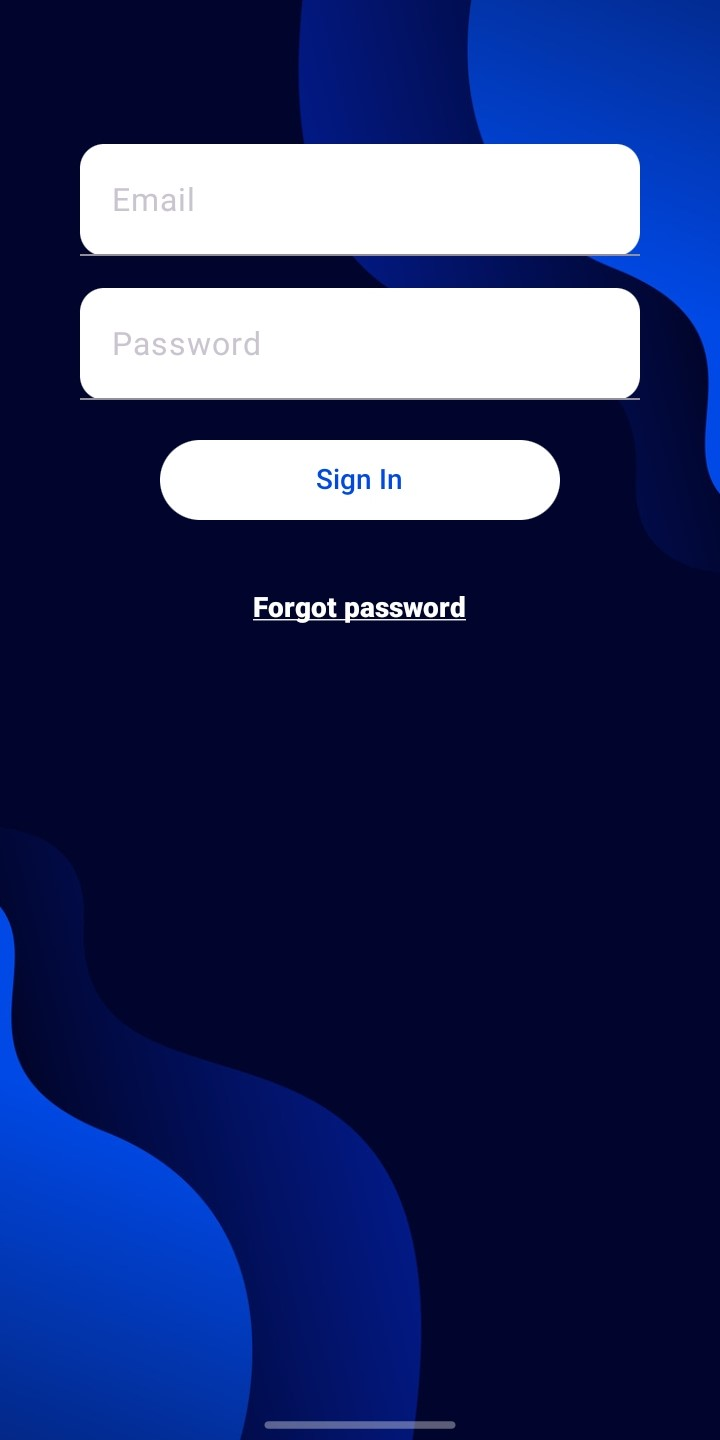
\includegraphics[width=\textwidth]{images/3-aplicatia-android/sign_in_screen.jpeg}
  \caption{}
  \label{fig:sign_in_screen}
  \end{subfigure}
  \begin{subfigure}{0.2\textwidth}
    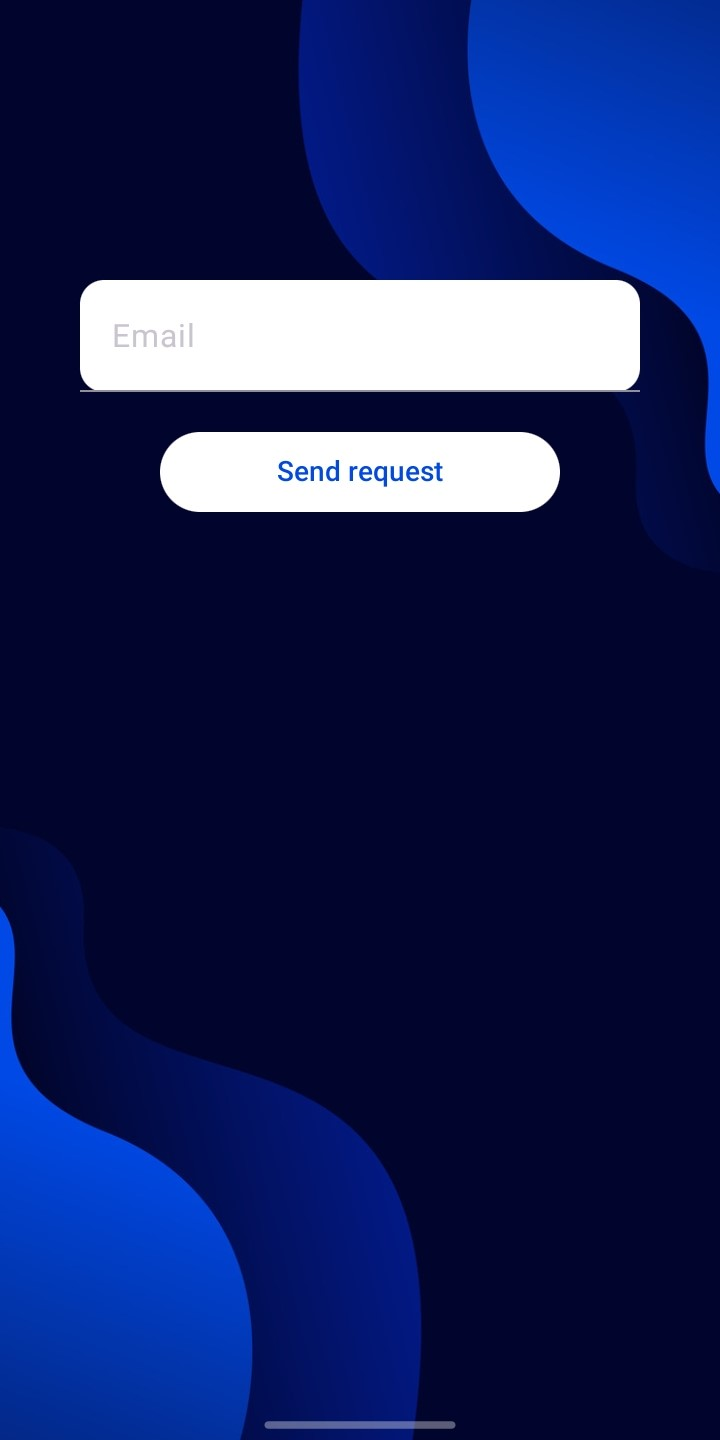
\includegraphics[width=\linewidth]{images/3-aplicatia-android/forgot_pass_screen.jpeg}
    \caption{}
    \label{fig:forgot_password}
  \end{subfigure}
  \caption[Conectare și resetarea parolei]{\textbf{Conectare și resetarea parolei}. \textit{(a) ilustrează câmpurile necesare pentru conectare (email și parolă), alături de butoanele Sign In pentru conectare și Forgot Password pentru resetarea parolei; (b) ilustrează ecranul pentru crearea unei cereri de restare a parolei.}}
  \label{fig:sign_up_validation_screens}
\end{figure}

\textbf{Meniul principal}. Meniul prezentat în Figura~\ref{fig:main_menu_screen} îi permite utilizatorului să aleagă între a învăța alfabetul ASL și a se deconecta. Deconectarea trimite o cerere către server pentru a invalida sesiunea și șterge token-urile prezente pe dispozitiv. Dacă utilizatorul apasă butonul \textit{Start learning}, camera se deschide și este inițiată o nouă sesiune de antrenament.

\textbf{Sesiune de învățare a alfabetului ASL}. Odată cu începerea unei sesiuni de antrenament, utilizatorul primește înștiințarea că este necesară introducerea mâinii în cadru (Figura~\ref{fig:start_learn_prompt}). Pe urmă, este afișată prima literă din alfabet, care rămâne pe ecran cât timp modelul nu recunoaște corect litera indicată (Figura~\ref{fig:learning_started}). Odată ce litera afișată este detectată, sesiunea continuă automat la următoarea literă din alfabet (Figura~\ref{fig:first_letter_detected}).

\begin{figure}[H]
\centering
    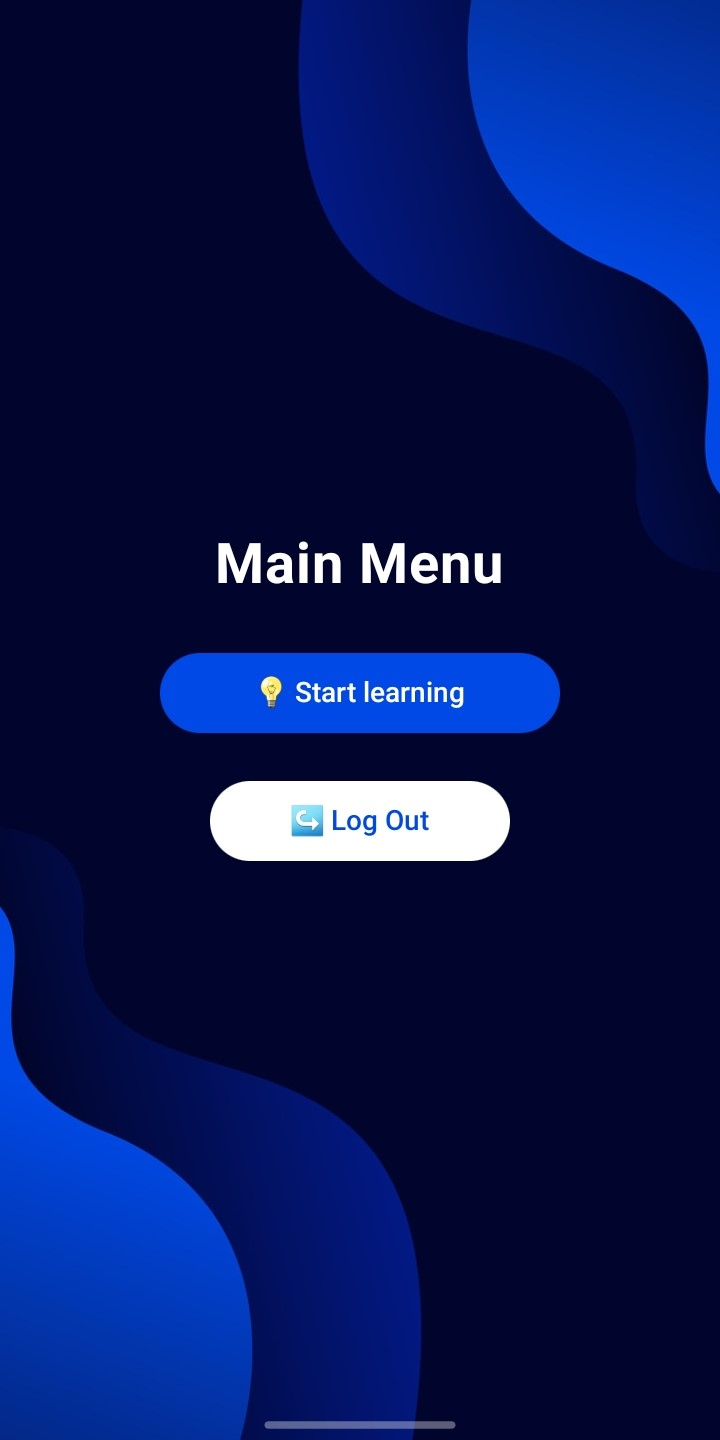
\includegraphics[width=0.2\textwidth]{images/3-aplicatia-android/main_menu_screen.jpeg}
  \caption[Meniul principal]{\textbf{Meniul principal}. \textit{Ilustrăm meniul principal care oferă opțiunile de începere a unei sesiuni de antrenament (Start Learning) și de decontectare (Log Out).}}
  \label{fig:main_menu_screen}
\end{figure}

\begin{figure}[H]
  \centering
    \begin{subfigure}{0.2\textwidth}
    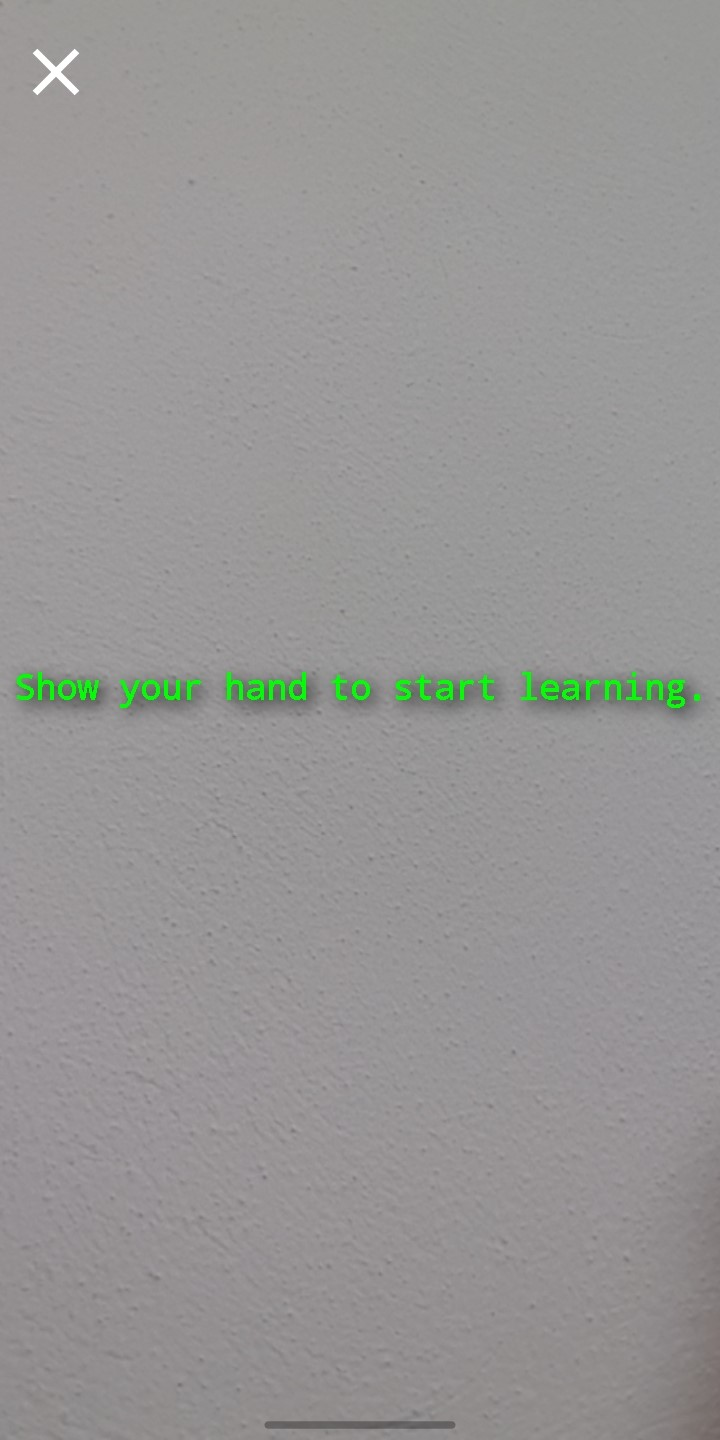
\includegraphics[width=\textwidth]{images/3-aplicatia-android/start_learn_screen.jpeg}
  \caption{}
  \label{fig:start_learn_prompt}
  \end{subfigure}
 \begin{subfigure}{0.2\textwidth}
    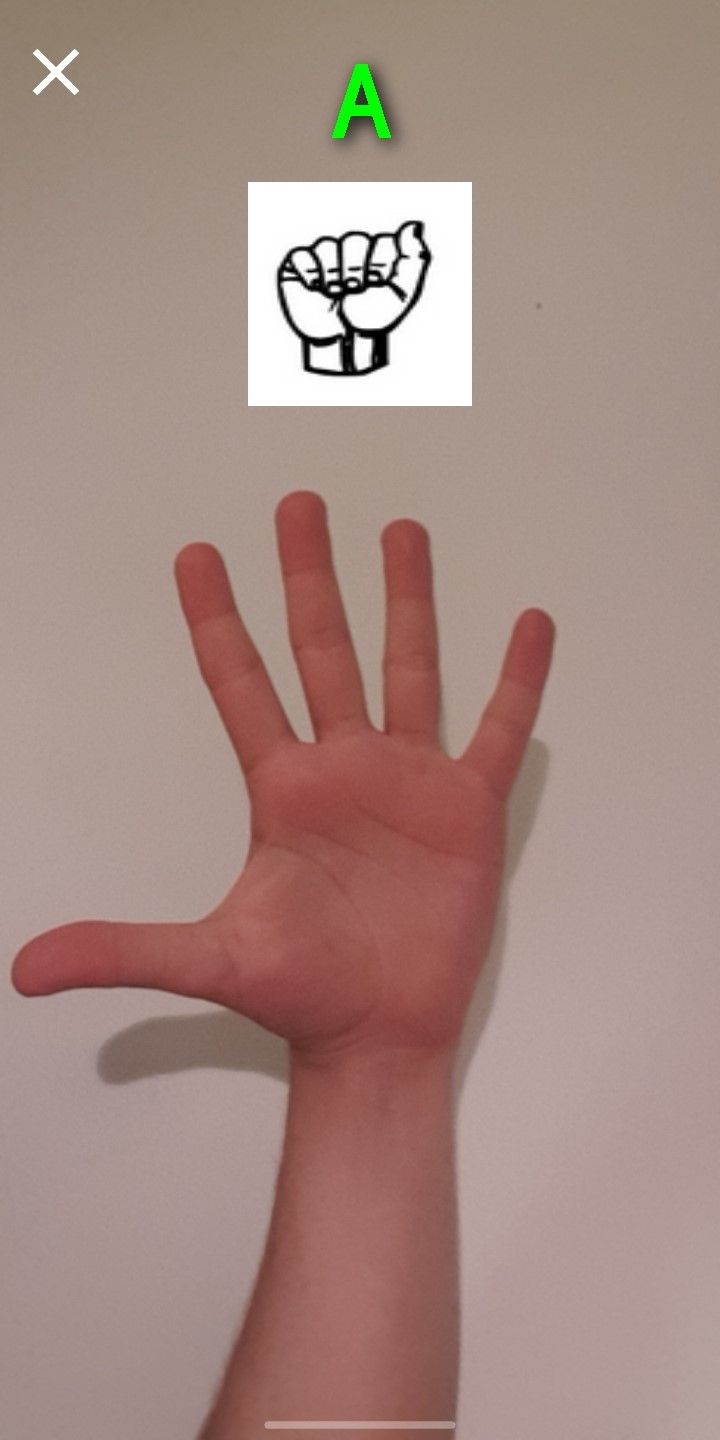
\includegraphics[width=\textwidth]{images/3-aplicatia-android/learning_started.jpeg}
  \caption{}
  \label{fig:learning_started}
  \end{subfigure}
   \begin{subfigure}{0.2\textwidth}
    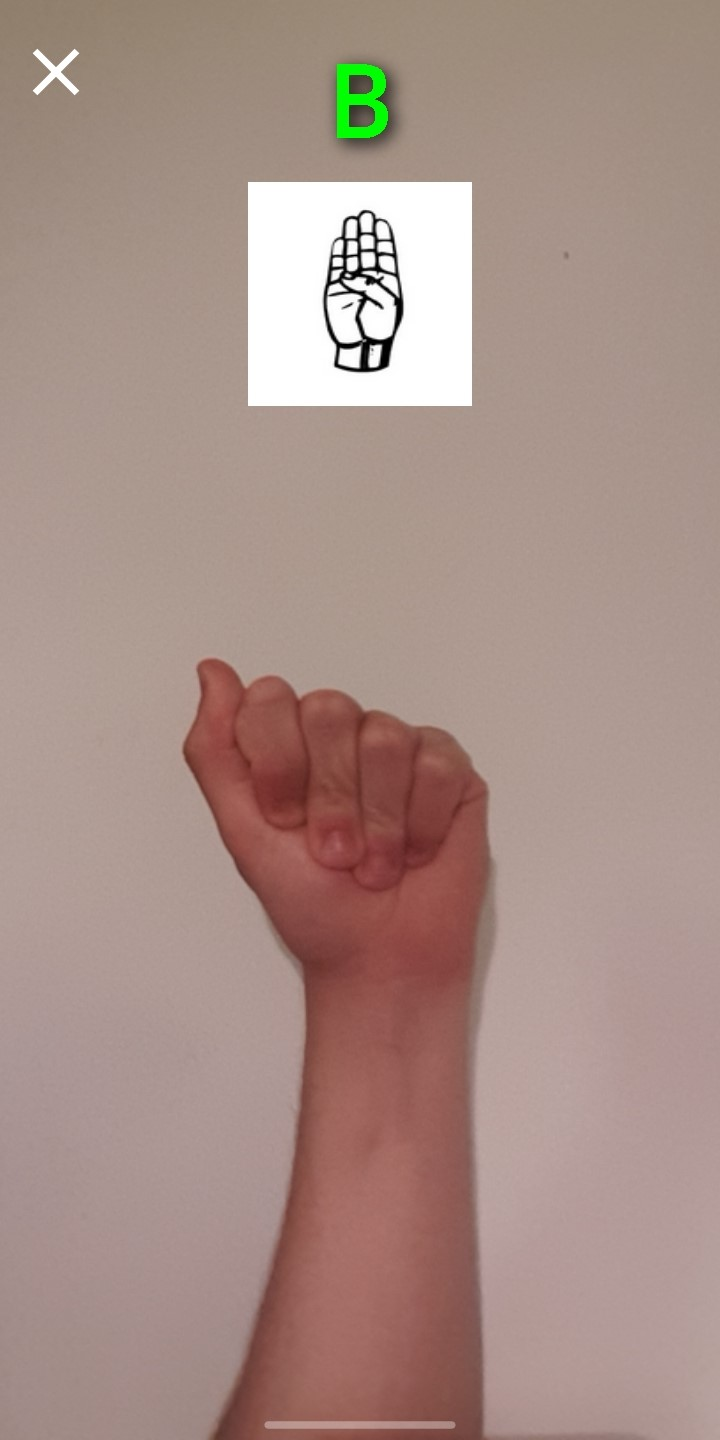
\includegraphics[width=\textwidth]{images/3-aplicatia-android/learn_a_detected.jpeg}
  \caption{}
  \label{fig:first_letter_detected}
  \end{subfigure}
  \caption[Sesiune de învățare]{\textbf{Sesiune de învățare}. \textit{(a) ilustrează instrucțiunea primită de utilizator pentru a își introduce palma în cadru; (b) ilustrează începerea sesiunii de învățare prin afișarea literei A; (c) ilustrează afișarea literei B. Utilizatorul află ce literă învață prin afișarea caracterului cu culoarea verde, iar dedesubt se află o imagine care ilustrează semnul pentru acea literă.}}
  \label{fig:training_sesh_figs}
\end{figure}

\section{Infrastructura aplicației}
\label{sec:server_app}
Arhitectura aplicației urmează o structură containerizată folosind \textbf{Docker} \cite{docker}, prin \textit{docker-compose}, ceea ce oferă un mediu de execuție portabil și izolat. Aplicația are la bază 4 containere:

\begin{itemize}
    \item \textbf{Uvicorn} + \textbf{FastAPI} - server asincron \cite{uvicorn} care răspunde cererilor HTTP prin cadrul de dezvoltare \textbf{FastAPI} \cite{fastapi}, care gestionează logica aplicației și oferă suport în gestionarea măsurilor de securitate.
    \item \textbf{PostgreSQL} - bază de date relațională, care asigură stocarea persistentă a datelor \cite{postgresql}.
    \item \textbf{Redis} - bază de date în memorie care funcționează pe bază de cheie-valoare \cite{redis} și asigură accesul rapid asupra datelor.
    \item \textbf{NGINX} - reverse proxy \cite{nginx} care preia cererile HTTP și le redirecționează către serverul Uvicorn, gestionează traficul și asigură conexiuni securizate prin \textit{SSL}.
\end{itemize}

\textbf{Server}. Serverul are la bază o arhitectură orientată pe servicii (SOA), structurată în straturi decuplate în funcție de responsabilitate. O cerere HTTP parcurge un flux logic de tipul: \textbf{API} \rightarrow \space\textbf{serviciu} (logica aplicației) \rightarrow\space \textbf{CRUD} (acces la baza de date) \rightarrow\space răspuns.

Conexiunea către baza de date este creată utilizând componenta de acces la baza de date în mod asincron oferită de biblioteca \textbf{asyncpg} \cite{asyncpg}, iar relația dintre entitățile bazei de date și modelele relaționale definite în cod este facilitată de biblioteca \textbf{SQLModel} \cite{sqlmodel}.

Relația de dependență dintre servicii este facilitată de clasa \textit{Depends} din biblioteca FastAPI, care asigură mecanismul de injectare a dependențelor. De exemplu, clasa \textit{AuthService} este injectată în \textit{endpoint}-urile pentru autentificare, iar clasele \textit{UserService} și \textit{RedisClient} sunt injectate în clasa AuthService, aceasta din urmă depinzând de cele două.

Pe lângă înregistrarea de conturi noi și capacitatea de a conecta și deconecta utilizatori de la aplicație, serverul are ca funcționalități și schimbarea parolelor și reîmprospătarea token-urilor de acces.

Pentru procesarea unei cererei de înregistrare, este validată adresa de email  cu ajutorul bibliotecii \textbf{email-validator} \cite{email_validator}. În urma validării, se verifică lipsa adresei în baza de date și a potrivirii textelor introduse în cele două câmpuri desemnate parolei. În continuare, se aplică o funcție de dispersie (în engl. \textit{hash}) asupra parolei cu ajutorul bibliotecii \textbf{bcrypt} \cite{bcrypt}, iar datele utilizatorului sunt salvate. În final, este generat un cod unic de verificare care este trimis printr-un email către utilizator, cu scopul de a verifica adresa de email. Adresa și codul de verificare sunt salvate ca pereche cheie-valoare, unde codul reprezintă cheia și emailul reprezintă valoarea, într-o bază de date Redis, cu timp de expirare de cinci minute. Utilizatorul nu poate folosi datele sale de acces până nu confirmă adresa de email.


În urma validării contului de email, utilizatorul se poate conecta la noul său cont, moment în care sunt verificate datele sale de autentificare. Alături de un răspuns pozitiv, serverul trimite și un obiect de tip \textit{AuthorizationTokens}, care conține un token de acces și un token de reîmprospătare.

Pentru deconectare, clientul trimite către server token-ul de acces salvat pe dispozitiv și token-ul de reîmprospătare asociat. În cazul validării token-ului de acces, token-ul de reîmprospătare este invalidat, iar utilizatorul este deconectat și redirecționat către ecranul de bun-venit.



\textbf{Token de acces și token de reîmprospătare}. Timpul de expirare a token-ului de acces este, în cazul nostru, de o oră, și este semnat cu o cheie secretă, pentru a ne asigura, la recepționare, că acesta nu a fost manipulat în vreun fel. Avantajele JWT provin din principiul lipsei de stare pe care îl respectă, acesta nefiind stocat pe serverul aplicației, ci doar pe dispozitivul utilizatorului.

Rolul token-ului de reîmprospătare este vizibil în momentul în care expiră JWT. Acesta este stocat în baza de date Redis și este folosit pentru crearea unui nou JWT. Tandemul token de acces - token de reîmprospătare oferă utilizatorului o experiență plăcută în navigarea prin aplicație, deoarece toate verificările sunt făcute în fundal, fără a fi necesare reconectări manuale frecvente. Token-ul de reîmprospătare este valabil, în cazul nostru, timp de 30 de zile, perioadă la finalul căreia utilizatorul trebuie să se conecteze din nou.

\textbf{Persistența datelor}. Stocarea datelor este facilitată de o bază de date relațională de tip PostgreSQL și de o bază de date în memorie, Redis.

Baza de date relațională este folosită pentru a salva datele utilizatorilor și conține o tabelă numită \textit{users}. Coloana \textit{id} este cheia primară, de tip \textit{UUID4}, \textit{email} și \textit{password} sunt de tip \textit{VARCHAR}, iar \textit{confirmed} este de tip \textit{boolean} și asigură confirmarea contului.


Pentru a avea o experiență fluentă în utilizarea aplicației, am optat pentru stocarea token-urilor de reîmprospătare și a codurilor de acces într-o bază de date Redis. Token-urile de reîmprospătare, codurile de validare a adreselor de email și cele pentru schimbarea parolelor sunt accesate cu un timp de latență minim. Toate cheile sunt salvate după ce au fost schimbate de o funcție hash, pentru a spori securitatea.

\textbf{Reverse proxy}. Toate cererile ajung mai întâi la containerul pentru NGINX, care le filtrează în funcție de cerințele notate în fișierul pentru configurări. În primul rând, sunt acceptate doar cereri HTTPS, containerul utilizând un certificat SSL. NGINX primește cereri la adresa \url{https://localhost:443}. De asemenea, am implementat un mecanism de limitare a numărului de cereri din partea unui singur utilizator, pentru a descuraja trimiterea unui număr ridicat de cereri într-un interval scurt. În urma filtrării, acestea sunt redirecționate către \url{http://uv-app:8000}, unde \textit{uv-app} este numele containerului care rulează serverul Uvicorn.